\documentclass[a4paper, 14pt]{extreport}
\usepackage[T2A]{fontenc}
\usepackage[utf8]{inputenc}
\usepackage[english, russian]{babel}
\usepackage{indentfirst}
\usepackage{setspace}
\usepackage{titlesec}
\usepackage{subcaption}
\usepackage{hyperref}
\usepackage{graphicx}
\usepackage[left=2.5cm, right=1.5cm, top=2.0cm, bottom=2.0cm]{geometry}

\graphicspath{{images/}}
\renewcommand{\rmdefault}{ftm}

\titleformat{\chapter}
    {\centering\normalsize}
    {\thechapter}
    {8pt}{\MakeUppercase}
\titleformat{\section}
    {\centering\normalsize}
    {\thesection}
    {1em}{}
\titleformat{\subsection}
    {\centering\normalsize}
    {\thesubsection}
    {1em}{}
\titlespacing*{\chapter}{0pt}{-30pt}{8pt}
\titlespacing*{\section}{\parindent}{*4}{*4}
\titlespacing*{\subsection}{\parindent}{*4}{*4}

\begin{document}
    \begin{titlepage}
        \begin{center}
            Министерство образования и науки РФ \\
            Государственное образовательное учреждение\\
            Высшего профессионального образования\\
            <<Волгоградский государственный технический университет>>\\
            Кафедра <<САПРиПК>>
        \end{center}
        \vspace{2.0cm}
        \begin{center}
            \large \textbf{ОТЧЁТ} \\
            по педагогической практике
        \end{center}
        \begin{flushleft}
            Студента\\
            Фамилия \underline{\hspace{5cm}} 
            Имя \underline{\hspace{5.1cm}}\\
            Отчество \underline{\hspace{5cm}}\\
            Факультет \underline{\hspace{4.8cm}} курс \underline{\hspace{2cm}} 
            группа \underline{\hspace{4cm}}\\
        \end{flushleft}
        \vspace{1.0cm}
        \noindentТема работы: \underline{\hspace{10cm}}
        \vspace{2.0cm}
        \begin{flushleft}
            РУКОВОДИТЕЛЬ ПРАКТИКИ\\
            Кафедра \underline{\hspace{5cm}} Должность \underline{\hspace{5cm}} \\
            Фамилия \underline{\hspace{4.9cm}} Имя \underline{\hspace{6.5cm}}\\
            Отчество \underline{\hspace{4.9cm}}
        \end{flushleft}
        \vspace{1.5cm}
        \begin{flushright}
            <<\underline{\hspace{1.0cm}}>>\underline{\hspace{4.0cm}} \the\year г.
        \end{flushright}
        \vspace{\fill}
        \begin{center}
            Волгоград \the\year
        \end{center}
    \end{titlepage}
    \tableofcontents
    \onehalfspacing
    \chapter{Введение}
    OpenStreetMap -- некомерческий веб-картографический проект, который создаёт и предоставляет свободные 
    географические данные и возможность создавать карты всего мира кому угодно, кто это хочет.

    OpenStreetMap является подобием Википедии, только для веб-карт, которую может редактировать кто 
    угодно. Если магазин отсутствует на карте, его может добавить как владелец магазина, так и его 
    посетитель. Что касается показа карты, то любой человек или компания, принимающие участие в создании 
    карты, свободен рендерить её как ему удобно. Главная карта на \url{openstreetmap.org} использует 
    ПО рендеринга и стиль со свободной лицензией, которые кто угодно может взять и подправить под свои 
    нужды. Проще говоря, любой, кому необходимо, всегда может создать свои собственные карты, основываясь 
    на данных OSM.

    Также, несмотря на то, что самые популярные построители маршрутов для OpenStreetMap лицензированы под 
    FLOSS, даже если какая-нибудь компания и выберет другую лицензию, пользователи всегда могут использовать 
    свои построители маршрутов, и сравнив результаты построения, выявить какие-либо подтасовки, если они 
    есть.

    И наконец, пользователь волен скачать любую часть или даже всю карту OpenStreetMap для использования в 
    оффлайне. Это означает, что можно использовать данные OpenStreetMap для навигации, вообще не передавая 
    информацию о вашем местоположении на сторону.

    \chapter{Сбор информации}
    Информация по проекту OpenStreetMap и Leaflet была собрана из различных интернет источников. Самая 
    актуальная и достоверная информация, среди которой: структура, примеры использования, API, плагины 
    была непосредственно взять со страниц ресурсов. Дополнительная информация по работе, а также 
    разъяснение некоторых тонкостей в работе были взять со следующих сайтов:
    \begin{itemize}
        \item Хабрахабр -- многофункциональный сайт, представляющий собой смешение новостного сайта 
            и коллективного блога, созданный для публикации новостей, аналитических статей, мыслей, 
            связанных с информационными технологиями, бизнесом и Интернетом.\\
            \url{http://habrahabr.ru/}
        \item OpenStreetMap (OSM) -- некоммерческий веб-картографический проект по созданию силами 
            сообщества участников-пользователей Интернета подробной свободной и бесплатной 
            географической карты мира.\\
            \url{http://www.openstreetmap.org/}
        \item Leaflet -- современный Open-Source проектом для отображения мобильных 
            интерактивных карт.\\
            \url{http://leafletjs.com/}
        \item Wikipedia -- свободная общедоступная мультиязычная универсальная 
            интернет-энциклопедия, реализованная на принципах Вики.\\
            \url{https://ru.wikipedia.org}
    \end{itemize}
    К одним из основных источников информации можно причислить и Хабрахабр, так как в его тематических 
    блогах имеется большое количество информации предоставляющее подробное объяснение по тому или иному 
    вопросу. Стоит также выделить хороший стиль подачи информации и подкрепление текста визуальной 
    информацией.

    \chapter{Структура методического пособия}
    В структуре методического пособия были выделены следующие пункты:
    \begin{enumerate}
        \item Введение
        \item OpenStreetMap
        \begin{enumerate}
            \item Общие сведения
            \item История возникновения и развития
            \item Возможности платформы
            \item Формат данных
            \begin{enumerate}
                \item Базовые типы географических данных в OpenStreetMap
                \item Информационная схема объектов
                \item Геометрические примитивы
            \end{enumerate}
        \end{enumerate}
        \item Leaflet
        \begin{enumerate}
            \item Введение
            \item Возможности библиотеки
            \item Примеры работы с библиотекой
            \begin{enumerate}
                \item Подготовка HTML-страницы
                \item Создание карты
                \item Маркеры, круги и всплывающие сообщения
                \item Ломанная и область
            \end{enumerate}
        \end{enumerate}
        \item Задания
        \item Контрольные вопросы
        \item Ссылки и примечания
    \end{enumerate}

    \newpage

    В разделах \emph{Введение} даётся общее описание системы, история возникновения и развития. В разделах 
    связанных с \emph{возможностями} предоставляемые системой описаны специфические параметры стабильных 
    версий, которые доступны разработчику на данный момент. В разделе \emph{формат данных} проекта 
    OpenStreetMap описана техническая реализация данных, которые предоставляются разработчику, а также 
    пояснения по работе с ними. В разделе \emph{примеры работы с библиотекой} Leaflet представлены исходные 
    коды и пояснения к ним, а также графическое представление исполненного кода. В нём подробно рассмотрено 
    создание интерактивных карт используя простой в реализации программный код на языке JavaScript. 
    В последних нескольких разделах представлены задания, вопросы и ссылки.

    Методическое пособие доступно по следующей ссылке \url{https://github.com/vstu-cad-stuff/osm-manual}

    \chapter{Скриншоты}
    \begin{figure}[ht!]
        \center
        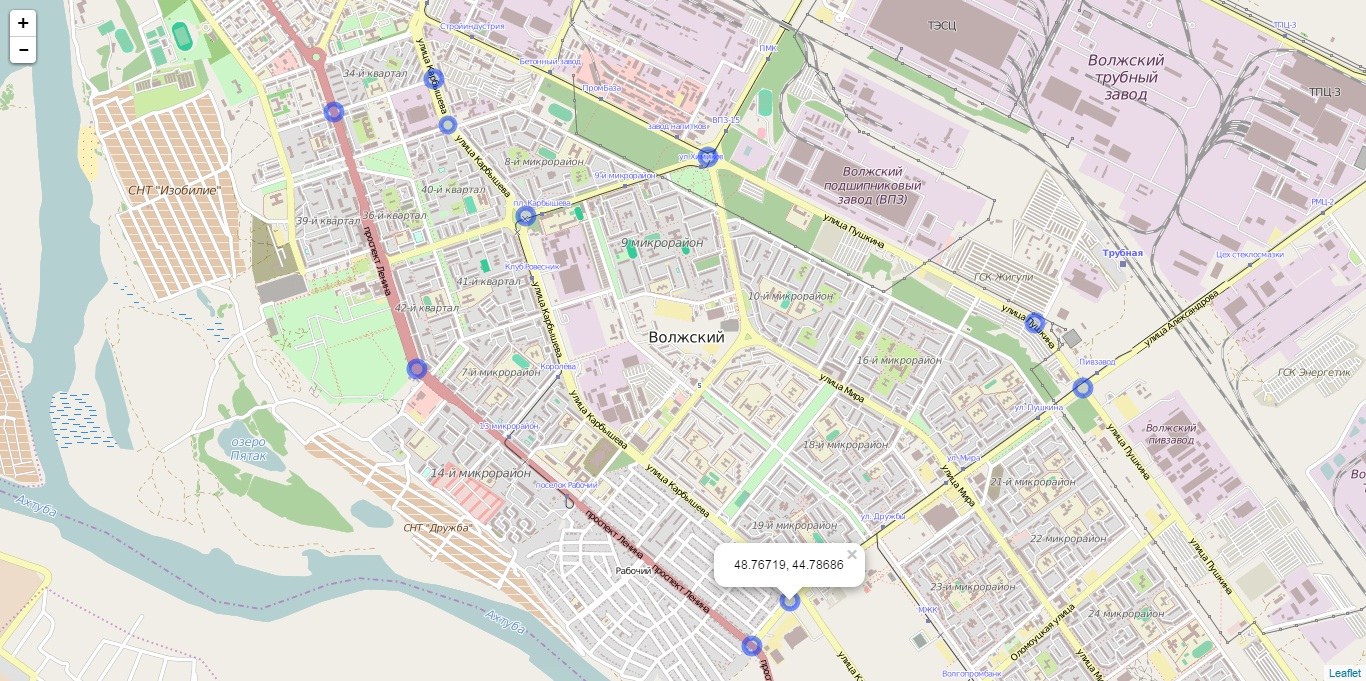
\includegraphics[width=0.9\textwidth]{e1}
        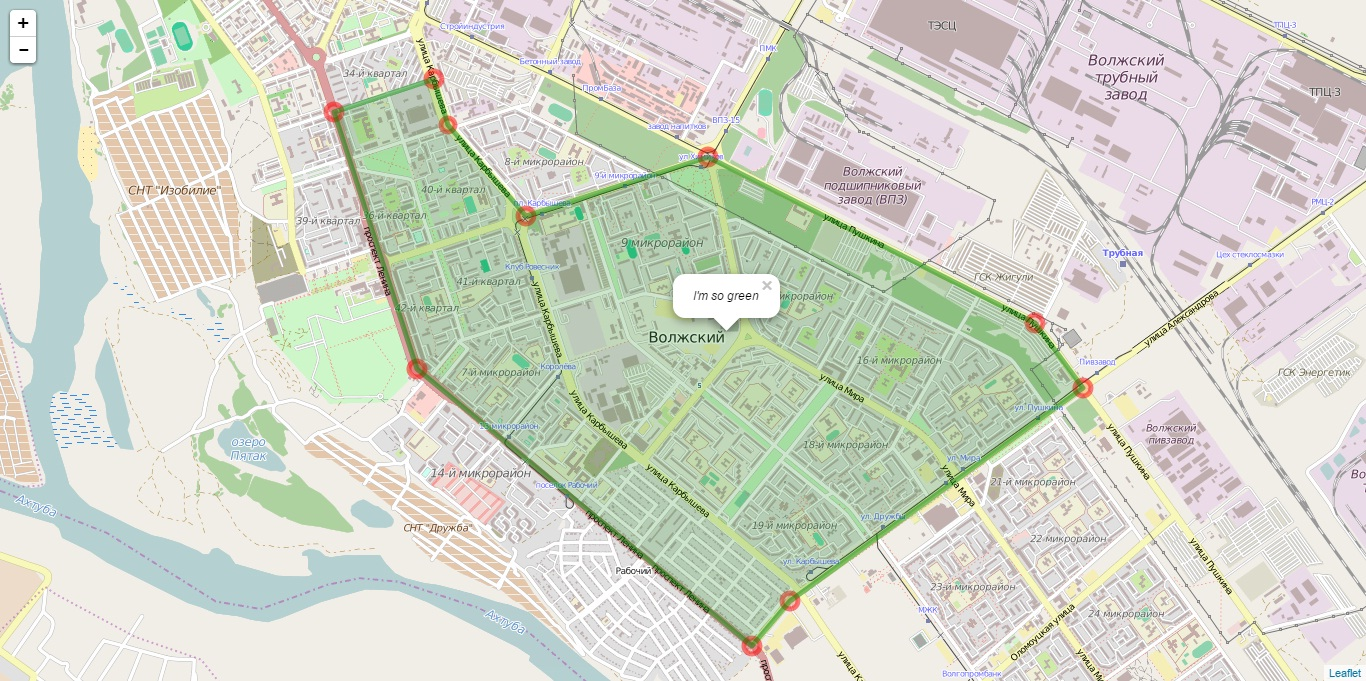
\includegraphics[width=0.9\textwidth]{e2}
        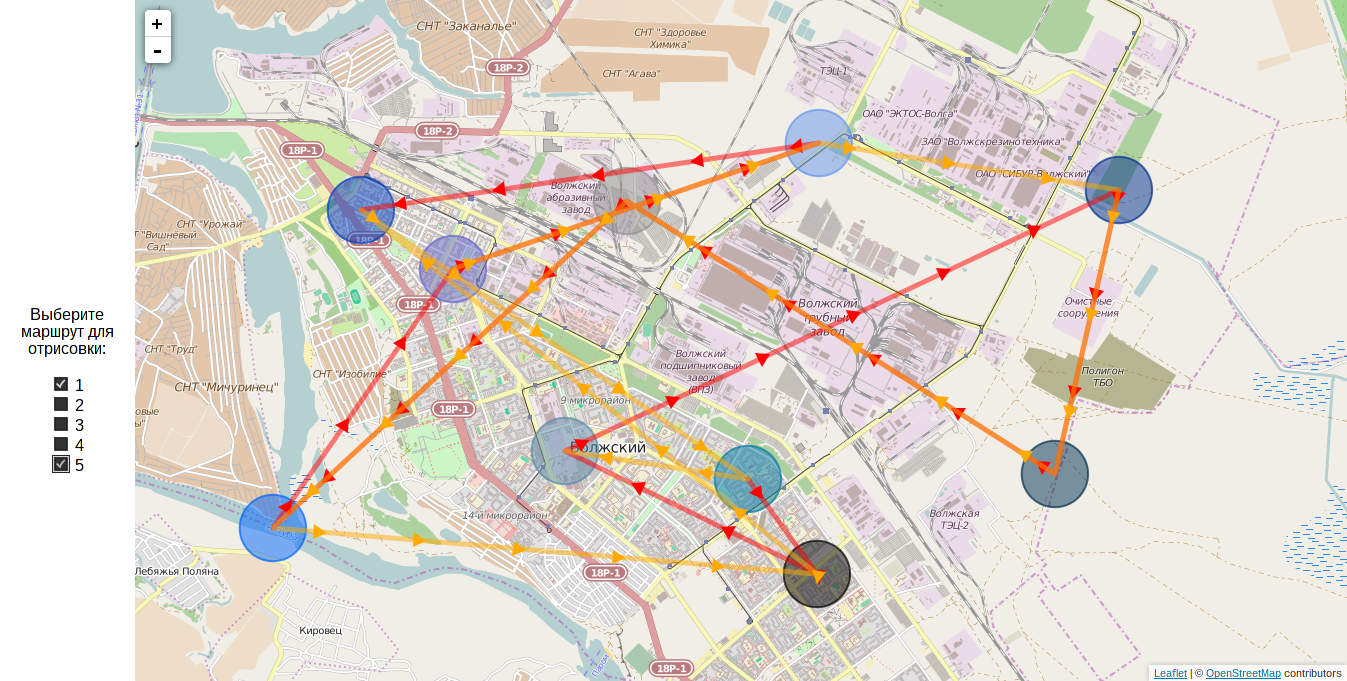
\includegraphics[width=0.9\textwidth]{e3}
    \end{figure}

    \chapter{Используемые технологии}
    Для проектирования и вёрстки были использованы следующие свободно распространяемые программные 
    продукты:
    \begin{itemize}
        \item Arch Linux -- это независимо разрабатываемый i686/x86-64 дистрибутив GNU/Linux общего 
            назначения, достаточно гибкий для выполнения любой роли.\\
            \url{https://www.archlinux.org/}
        \item \TeX -- система компьютерной вёрстки, разработанная американским профессором информатики 
            Дональдом Кнутом в целях создания компьютерной типографии.\\
            \url{http://tug.org/}
        \item \LaTeX -- набор макрорасширений системы компьютерной вёрстки TeX.\\
            \url{http://www.latex-project.org/}
        \item Sublime Text 3 -- быстрый кроссплатформенный редактор исходных текстов программ.\\
            \url{www.sublimetext.com/3}
        \item GNU Image Manipulation Program (GIMP) -- растровый графический редактор, программа для 
            создания и обработки растровой графики и частичной поддержкой работы с векторной графикой.\\
            \url{http://www.gimp.org/}
        \item Mozilla Firefox -- свободный браузер на движке Gecko, разработкой и распространением 
            которого занимается Mozilla Corporation.\\
            \url{https://www.mozilla.org/}
        \item Git -- распределённая система управления версиями файлов. Проект был создан Линусом 
            Торвальдсом для управления разработкой ядра Linux, первая версия выпущена 7 апреля 2005 года.\\
            \url{http://git-scm.com/}
        \item GitHub -- самый крупный веб-сервис для хостинга IT-проектов и их совместной разработки. 
            Основан на системе контроля версий Git и разработан на Ruby on Rails и Erlang компанией 
            GitHub, Inc.\\
            \url{https://github.com/}
    \end{itemize}
\end{document}